\section{Discussion}
\label{sec:discussion}

The methodology of this study converged in a collection of results obtained through a research on the importance of maintaining a communication channel between parents and children, during distant-parenting situations. In the previous section, the results have been introduced in order to better define the sampled population. The aim of this section, on the other hand, is to construct from these objective results, our own hypotheses on the issue, by identifying the interesting patterns according to different features of the data (subsection \ref{subsec:analysis-results}). Then, we will discuss whether the obtained hypotheses could be transposed back to a Chinese context, seen for the LBC issue (\ref{transposability}). Lastly, we will draw an interview protocol, aimed to be helpful for a future field test in Mainland China, that could eventually bring to us the final prove, or disprove, to our hypotheses (\ref{interview-protocol}).

\subsection{Analysis of the results}
\label{subsec:analysis-results}

In this first part of the discussion, we aim to get a deeper understanding of the obtained results, that have been described in the previous section. The goal is to determine whether interesting patterns could be retrieved from the studied population, in accordance with the distant-parenting issue, and how this latter is faced by distant families.

As already mentioned while explaining the content of the survey (see section \ref{content-survey}), the literature review proposed substantial differences in the way the paternal or maternal figures dealt with distant parenting. Unfortunately, the data on the parent side is not sufficiently rich to draw a representative analysis and to determine whether similarities in our survey occurred. On the other hand, we might be interested in discovering unknown outlines on the child's side according to statistics (like age, gender, etc.) that have not been sufficiently explored yet.

\begin{figure}[H]
    \centering
    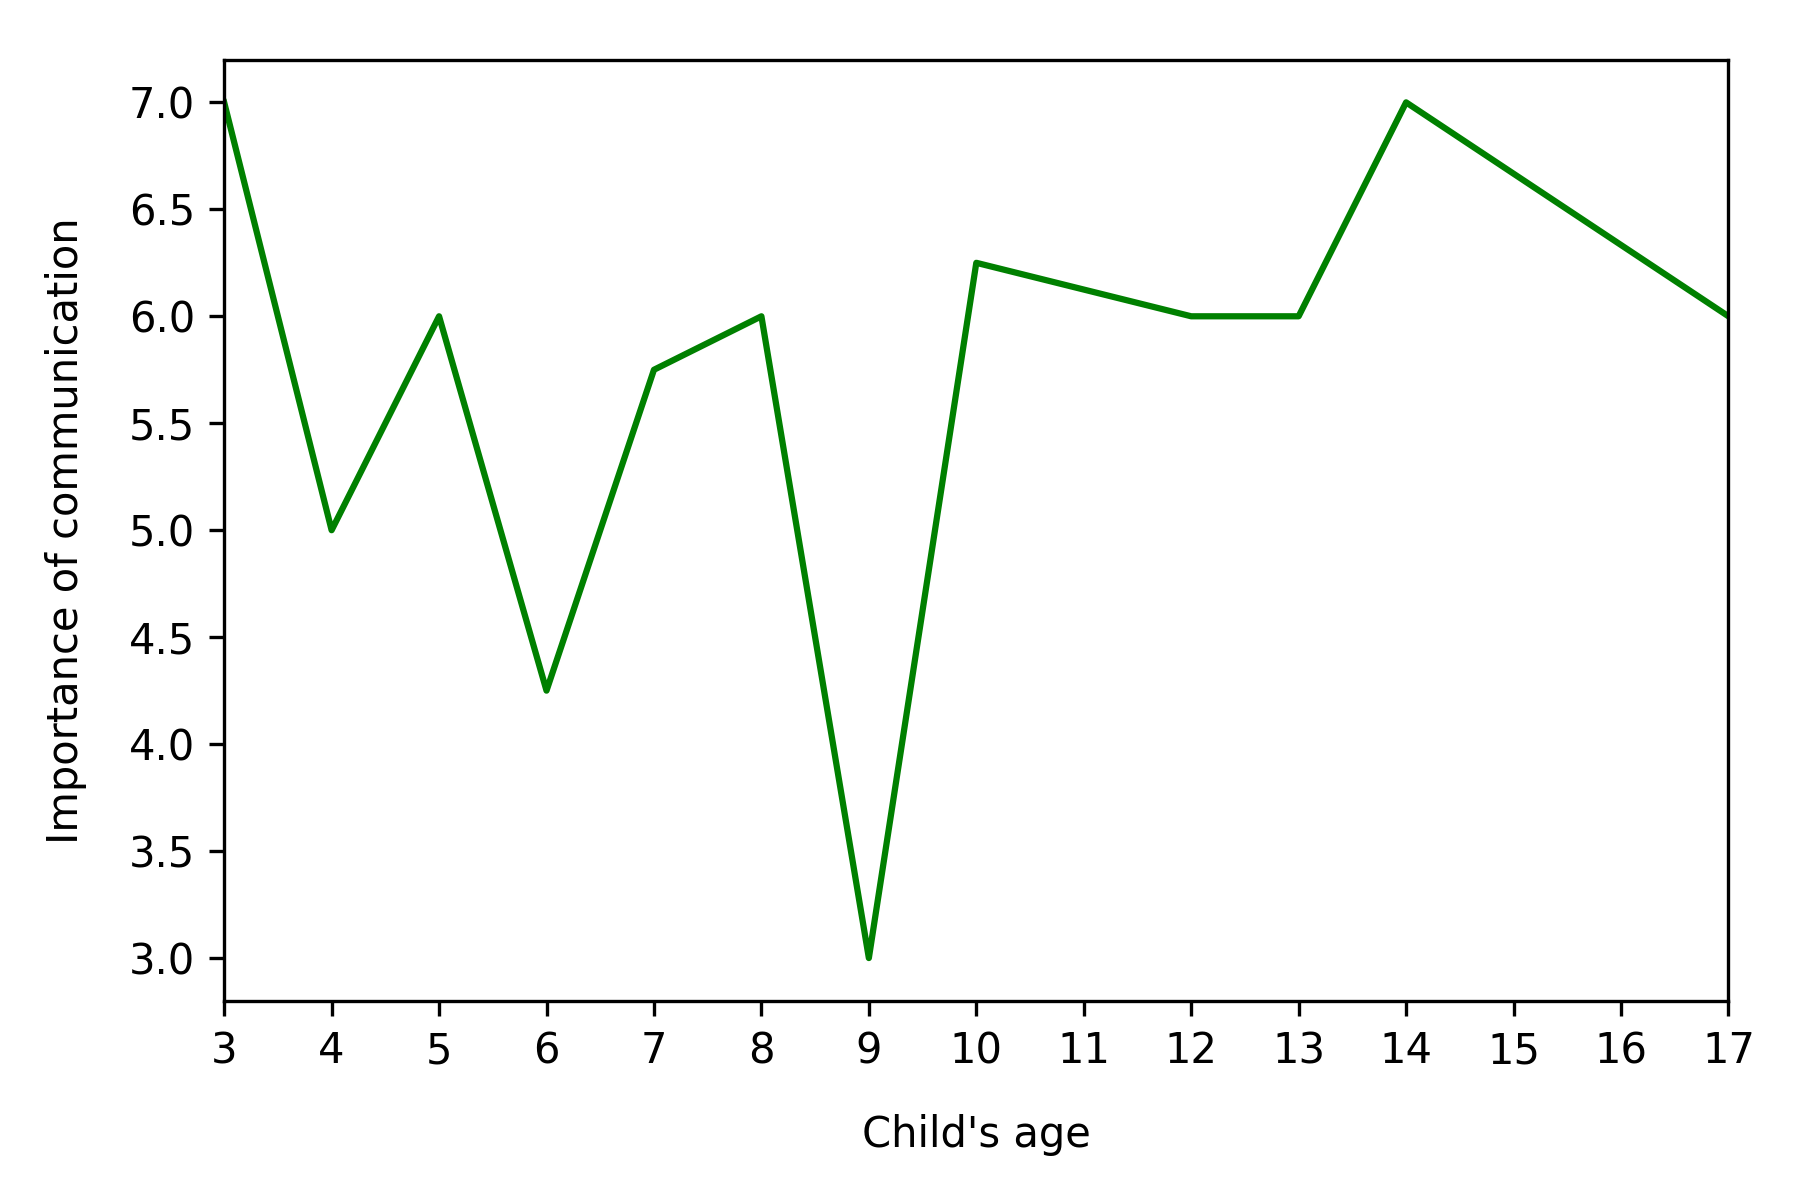
\includegraphics[scale=0.58]{plots/plot_1.png}
    \caption{Averaged importance of communication rated by the parents category, over child's age}
    \label{fig:plot_1}
\end{figure}

\begin{figure}[H]
    \centering
    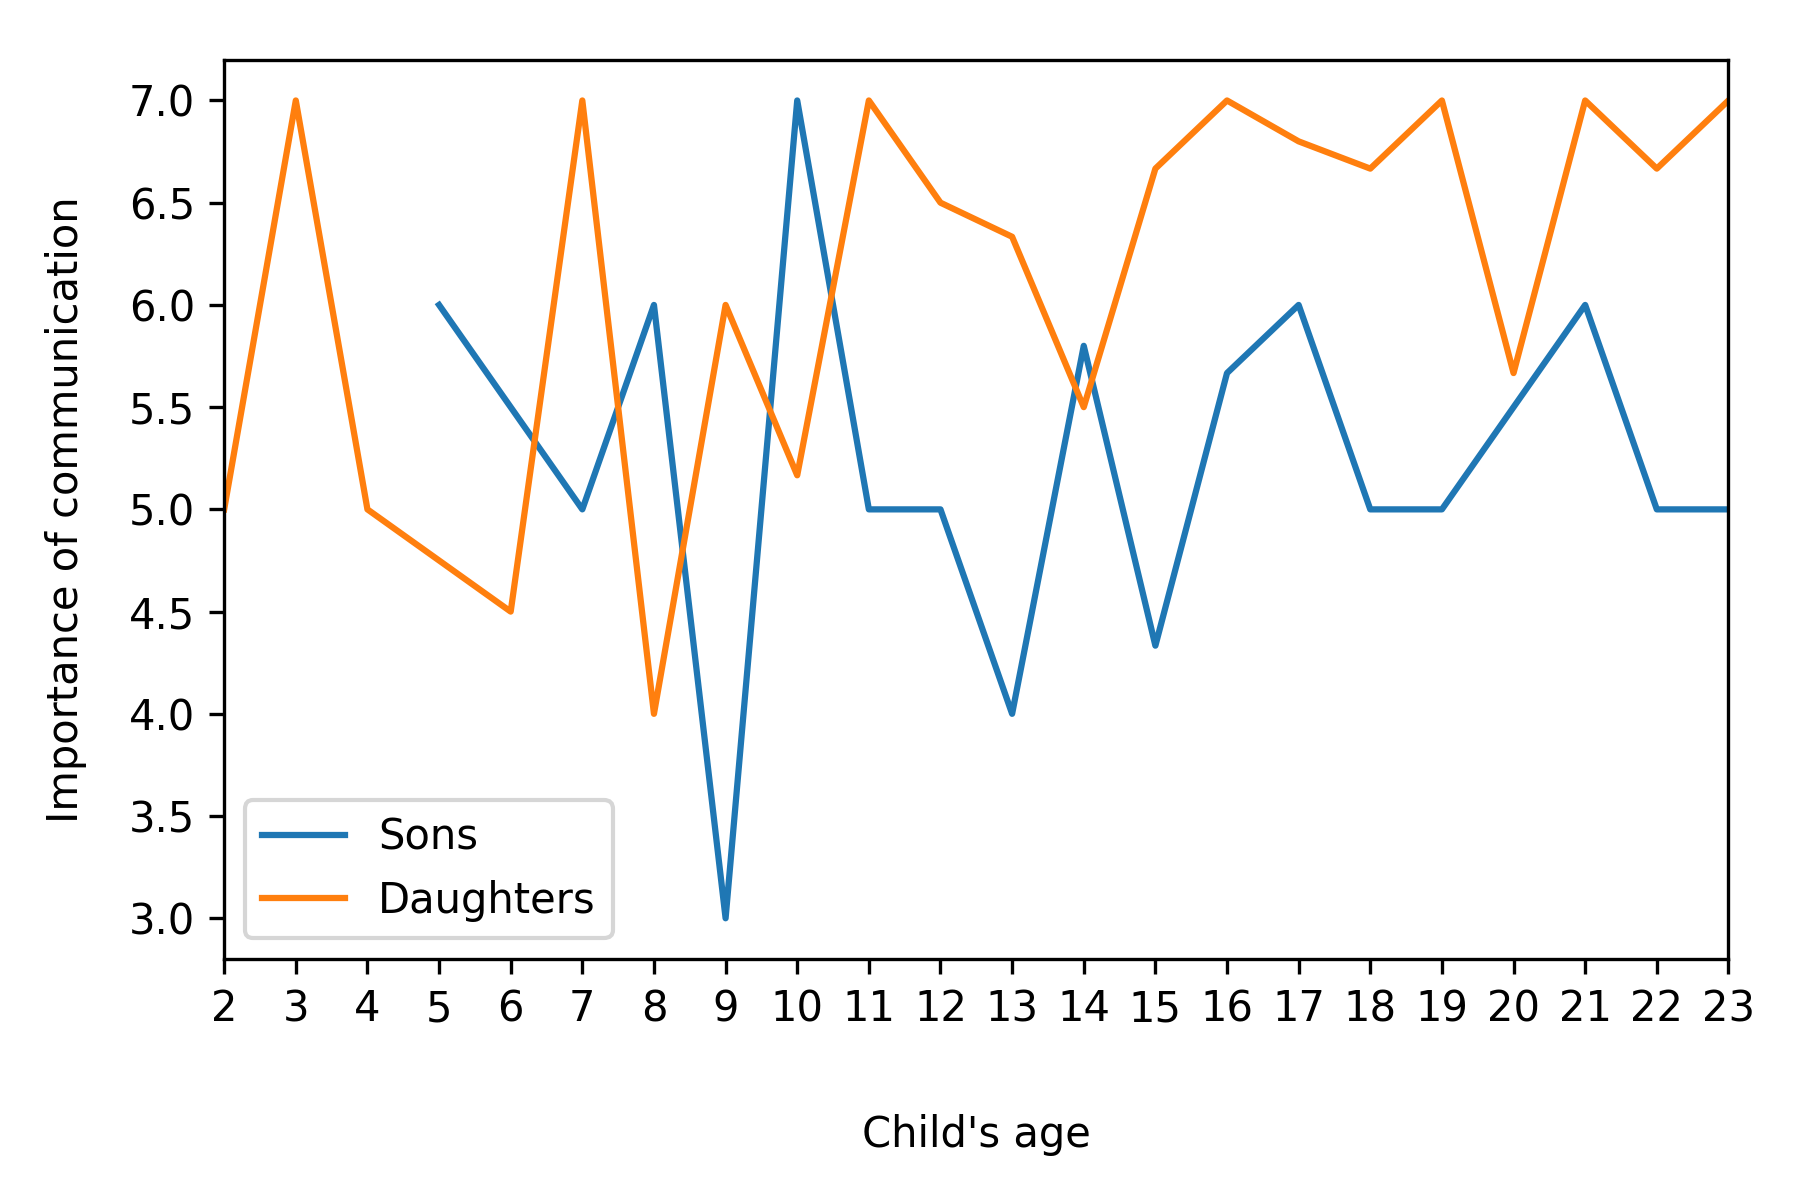
\includegraphics[scale=0.58]{plots/plot_2.png}
    \caption{Averaged importance of communication rated by the children category, over child's age}
    \label{fig:plot_2}
\end{figure}

The very first outcome from the collected data is about the feature regarding the importance of communication. We wanted to understand how the importance of communication was perceived, by both parents and children, and specifically how other factors might modify its trend. The two plots in figure \ref{fig:plot_1} and figure \ref{fig:plot_2} illustrate how the adoption of communication technologies (ICTs) are perceived by parents and children, according to different child's age during the distant-parenting experience. As already shown in the initial results (table \ref{tab:stats_children} and table \ref{tab:stats_parents}), the importance is generally perceived as extremely high, regardless of age differences. Although this latter might seem a trivial consideration, it is useful to keep in mind that such results are strongly related to the context from which they have been extrapolated and might be different in other social conditions and in other cultures, such as China. In order to avoid biases of any kind due to triviality in our own perspective, every result needs to be considered at this stage to later discuss it, in the Chinese context (see section \ref{transposability}).
Moreover, the two plots already illustrate the second consideration we can draw from the results. The trend clearly showcases a strong inclination of daughters, compared to same aged male peers, to give a higher weight to the importance of communication, from the age of ten years old (figure \ref{fig:plot_2}). Such results, therefore, suggests a possible exploratory pattern toward different responses according to child's gender and age, when being away from home for the very first time. 

The plot presented in figure \ref{fig:plot_3} tries to relate the frequency of communication with distant parents-children, according to different duration of the journey, during which the children spent time away from their families. The first intuition we had regarding a possible child's \textit{gender bias} in the data is confirmed by such plot. It generally illustrates a higher tendency for girls to have more frequent communication with their distant families, regardless of the duration of the experience. Would this trend suggest that daughters are more likely to consider communication more important than boys?

\vfill
\begin{figure}[H]
    \centering
    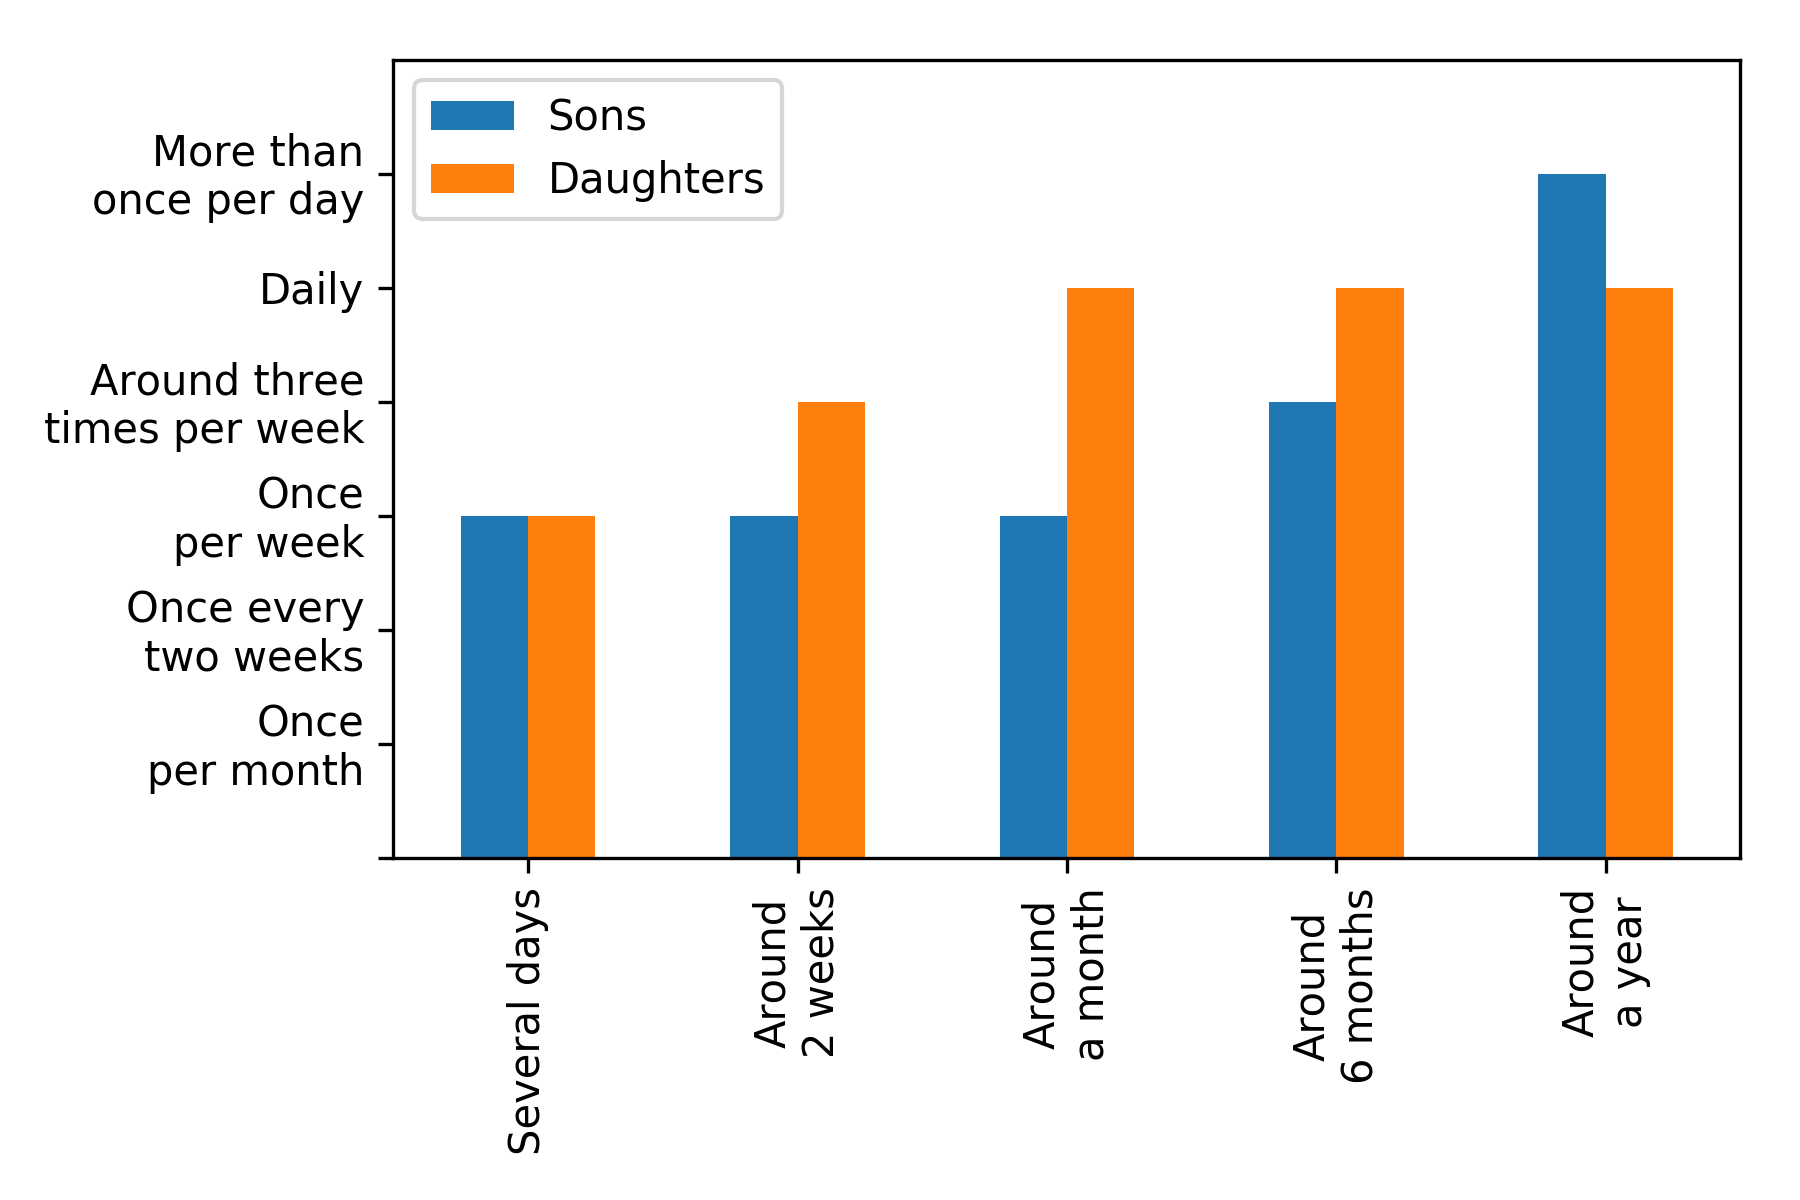
\includegraphics[scale=0.58]{plots/plot_3.png}
    \caption{Distribution of communication frequencies, over the duration of distant parenting}
    \label{fig:plot_3}
\end{figure}

Due to the amount of data collected, the exploratory analysis could be conducted on a higher granularity of distinct representative sets. This would allow to better understand what information the data contains and avoid falling in the possible trap of drawing conclusions from outliers. Firstly, we decided to project the data according to the duration of the distant-parenting experience, from both parents' and children's perspectives. We aim to determine whether the \textit{gender bias} trend could still be appreciated. Plots in figure \ref{fig:plot_7} and figure \ref{fig:plot_6} illustrate those findings from the children's and parents' point of view, respectively. We can indistinguishably see the same \textit{gender bias} trend, where girls perceive an higher importance of communication when staying away from their family (see figure \ref{fig:plot_7}). However, it is interesting to compare those results from the parents' perspective, where this trend is not prominent (see figure \ref{fig:plot_6}). The importance of communication for parents is generally not affected by the child's gender (nor the duration of the experience neither). Although the data-set collected from the parent side is far from being a reliable sample, results tend to be more homogeneous between  children’s gender (the only exception being a short-termed duration of several days), when compared to the child’s  perspective  illustrated  before. As already discussed previously, in the context from which such data has been collected, drawing a conclusion where parents consider equally important a communication channel with their children regardless of their gender might seem trivial. However, every result will be at last evaluated against the Chinese context, for which considerable amount of literature exists regarding gender discrepancies, mainly based on the \textit{One-Child Policy} of the past decades. Lastly, for the reader's interest, a plot illustrating the same data (from the parents' perspective), without any partitioning on features, can be found in the appendix \ref{appendix:additional-plots}.

\begin{figure}[ht]
    \centering
    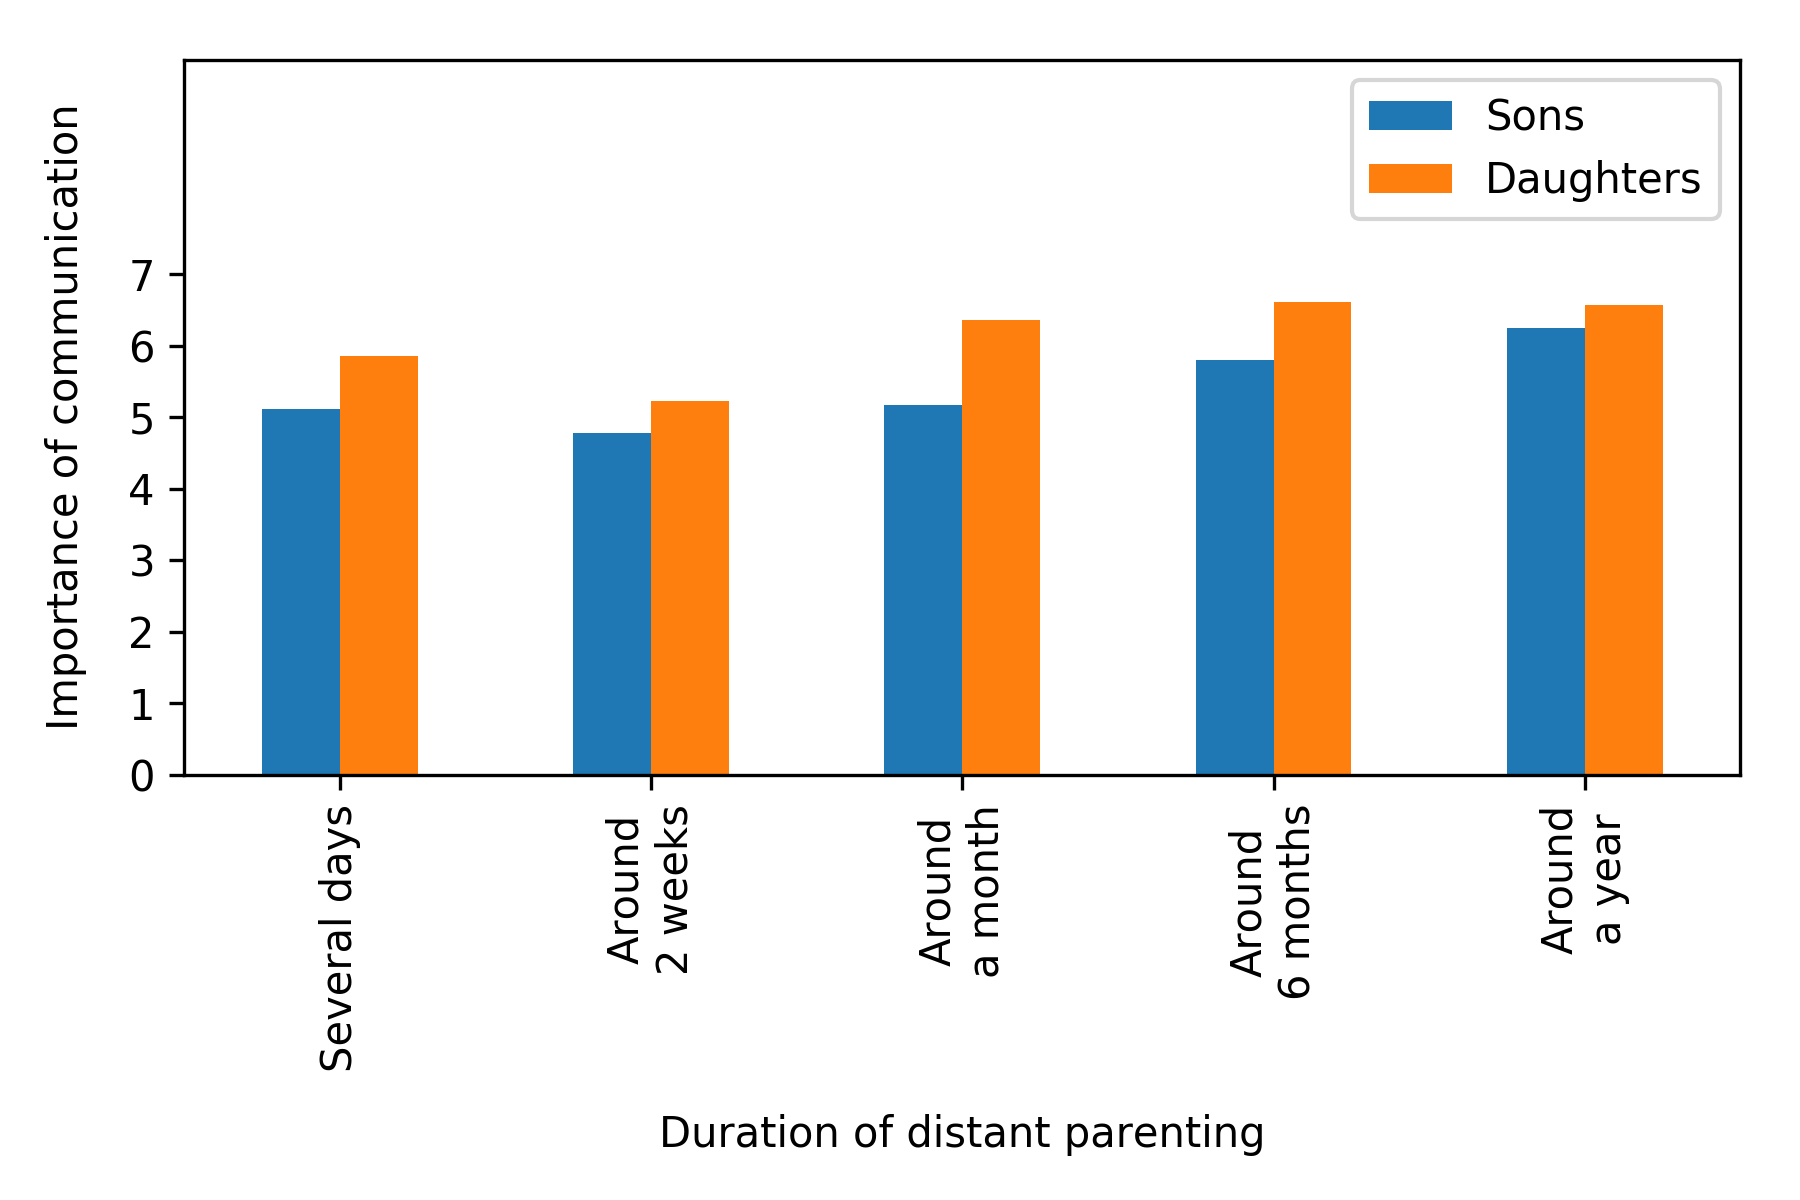
\includegraphics[scale=0.58]{plots/plot_7.png}
    \caption{Averaged importance of communication rated by the children category, over the duration of distant parenting}
    \label{fig:plot_7}
\end{figure}

\begin{figure}[ht]
    \centering
    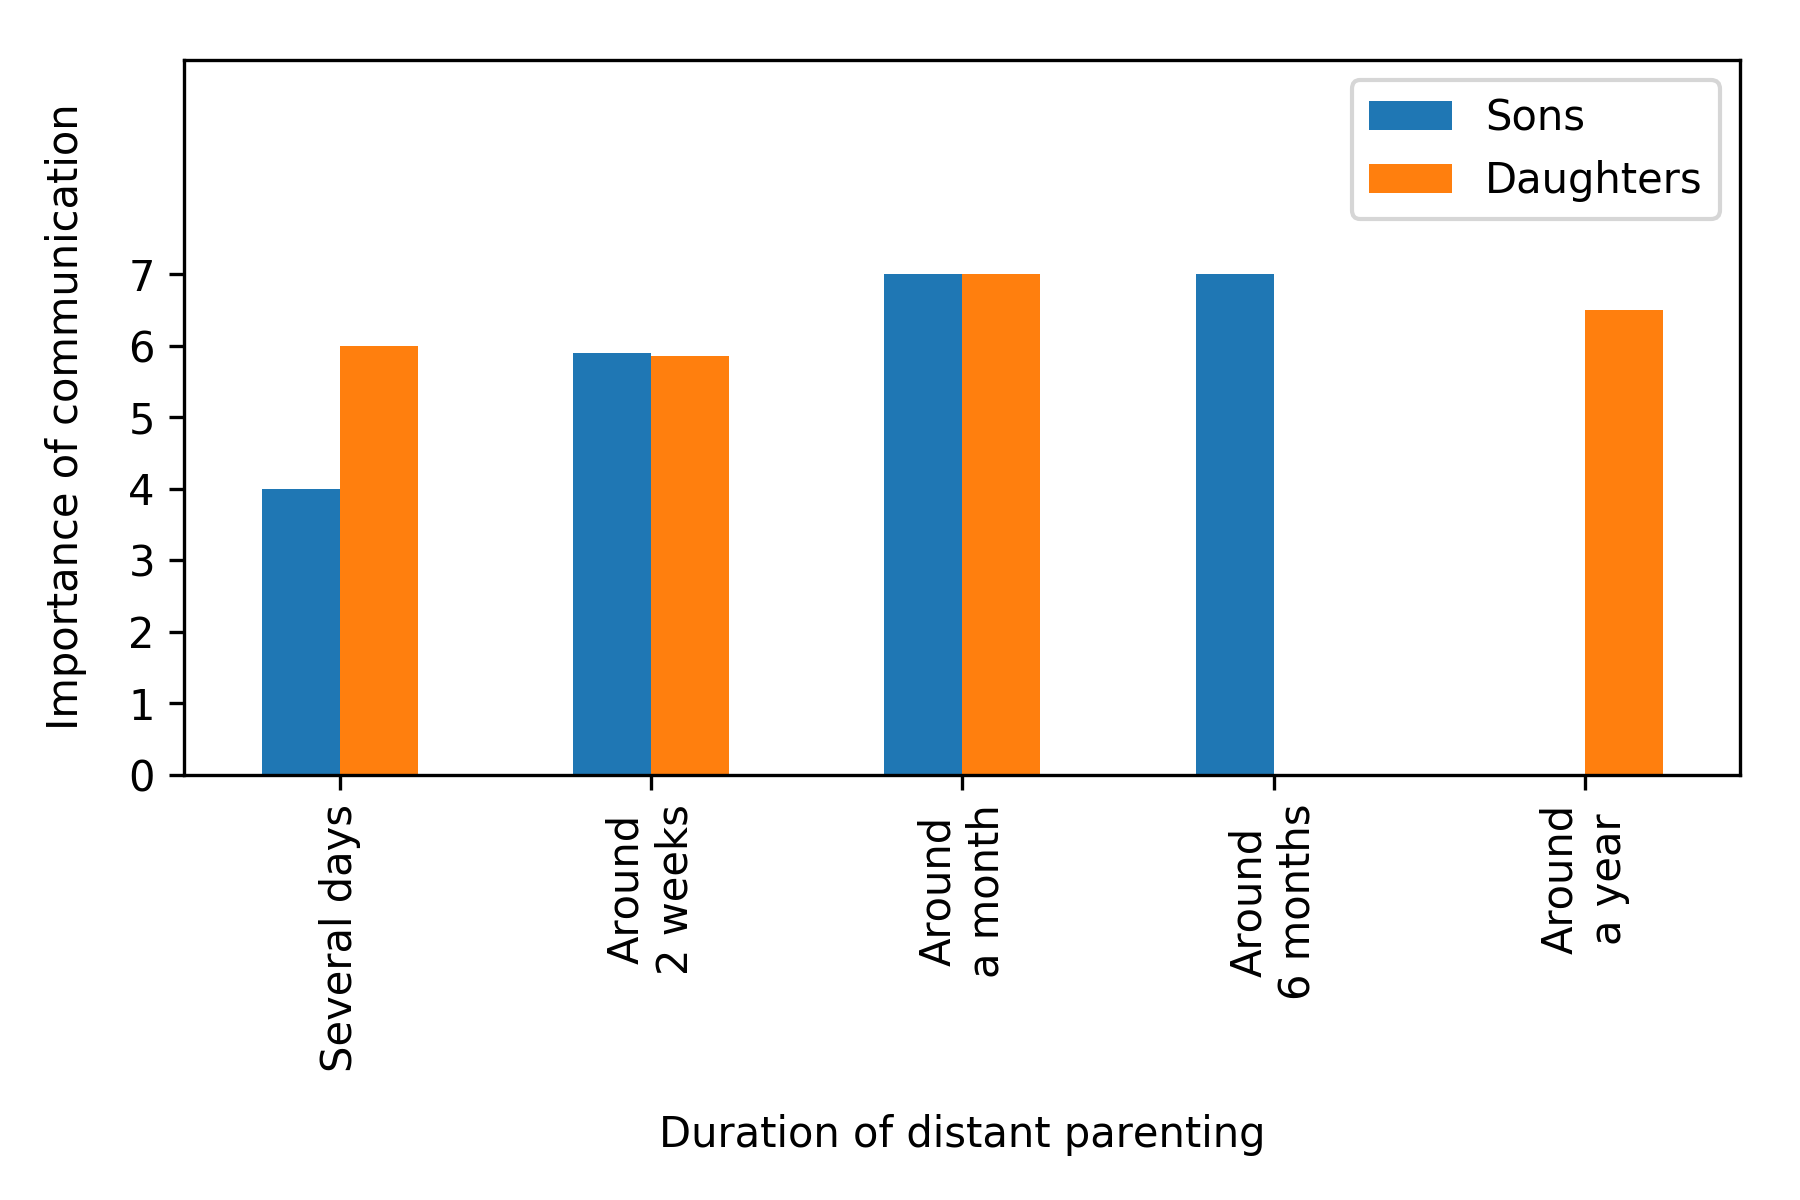
\includegraphics[scale=0.58]{plots/plot_6.png}
    \caption{Averaged importance of communication rated by the parents category, over the duration of distant parenting}
    \label{fig:plot_6}
\end{figure}
    
The same analysis from both the parents' and children's perspectives has been conducted on the \textit{Frequency of communication} factor base. This latter exploratory step, in conjunction with the previously computed plots, would help to better define discovered patterns on multiple variables, in order to detect variances in the data. The two plots illustrated in figure \ref{fig:plot_10} and figure \ref{fig:plot_9} showcase such distributions from the children's and parents' points of view, respectively. As previously proposed, an analysis on the parent data without partitioning, which does not present peculiarities to discuss, can be found in the appendix \ref{appendix:additional-plots}. Once again, there is a clear tendency for girls to express a much higher importance towards communication, regardless to how frequent distant families communicate throughout the experience. In short, the bias child's gender showcases, with respect to the communication, is once again confirmed. On the other hand, parents tend to not showcase any different behaviour according to their child's gender, reinforcing the hypothesis that a \textit{gender bias} would not exist on their point of view. However, it is interesting to underline how both plots (which are modelled around different sample groups, one for children and one for parents) identify a peculiar prominence for boys (or parents with a son) to higher rate the importance of communication, whenever the frequency of communication hits the "every other week" point. In order to draw solid conclusions about such peculiarity, an higher sampled population would be required to not mistake outliers for defined patterns.  

\begin{figure}[ht]
    \centering
    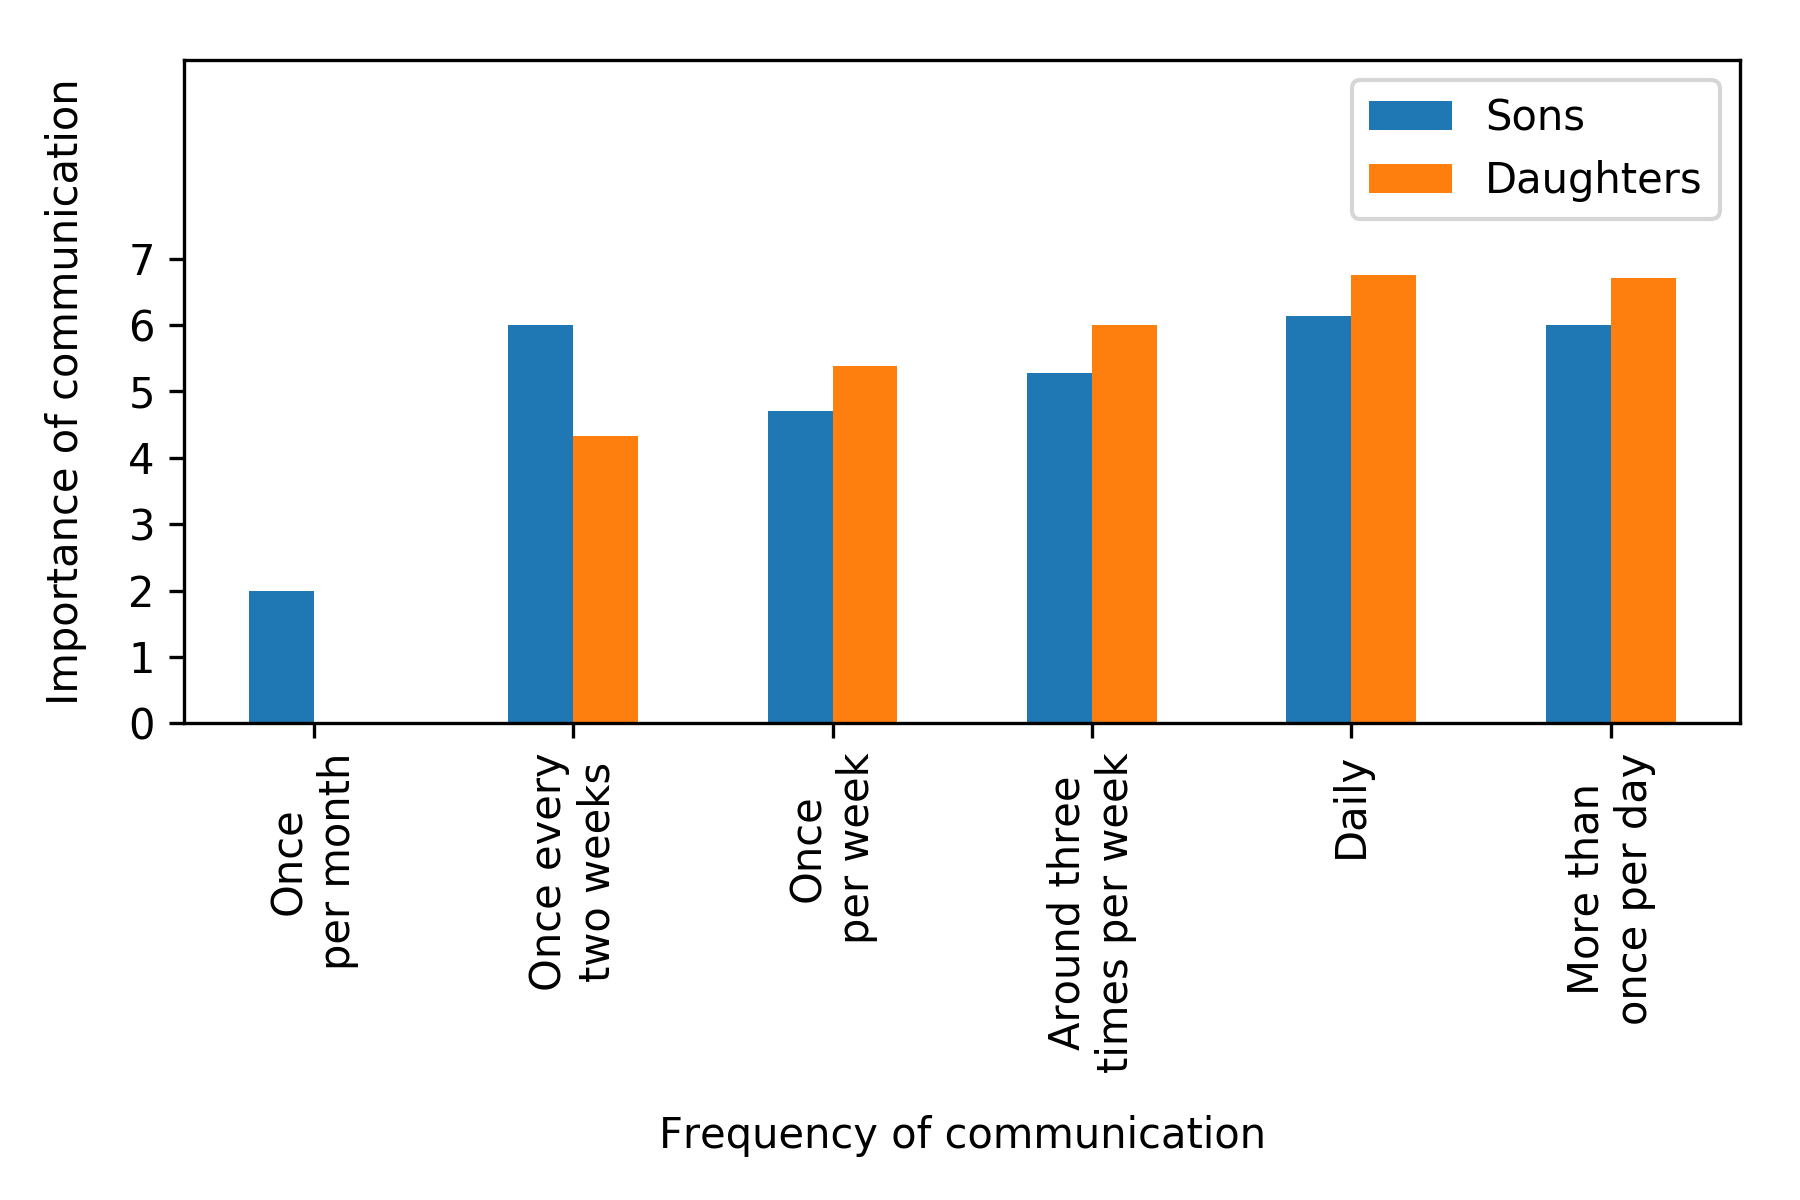
\includegraphics[scale=0.58]{plots/plot_10.png}
    \caption{Averaged importance of communication rated by the children category, over the frequency of communication}
    \label{fig:plot_10}
\end{figure}

\begin{figure}[ht]
    \centering
    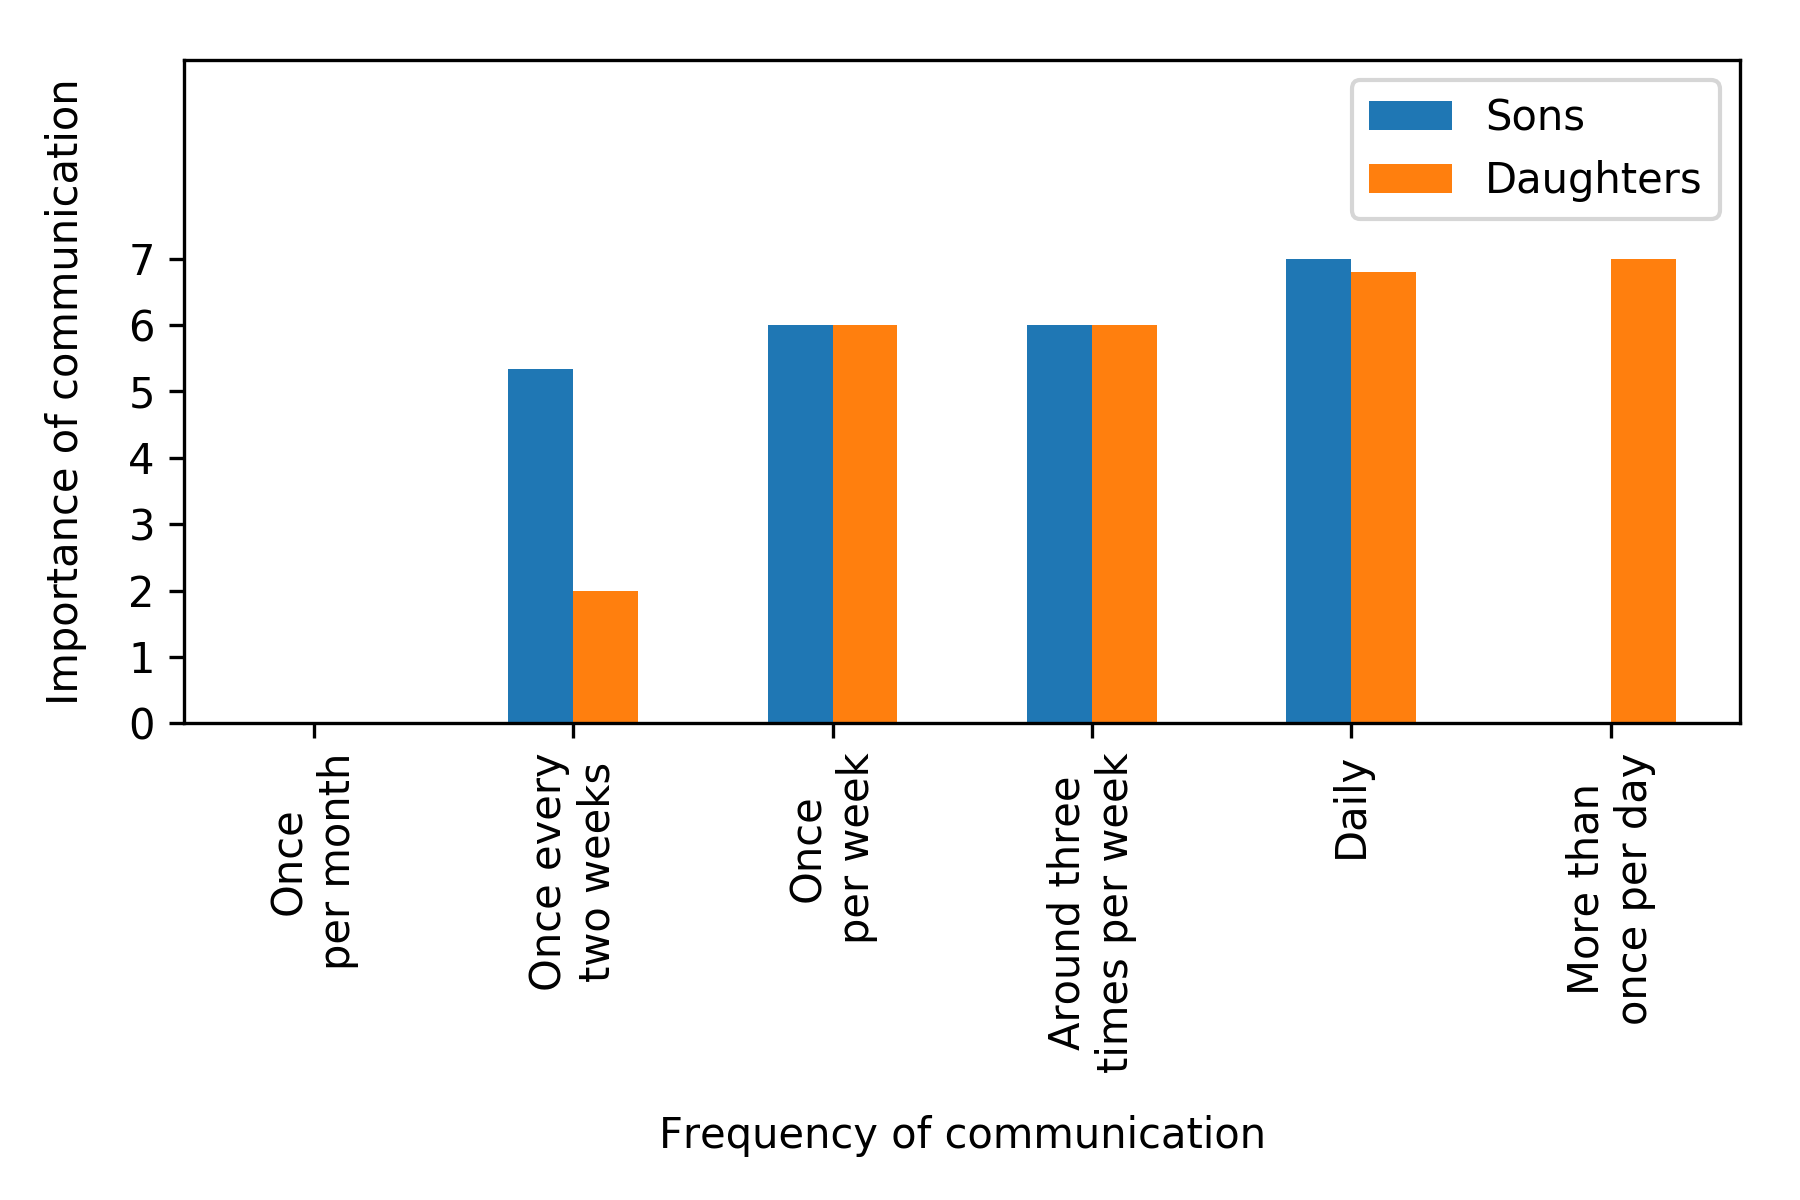
\includegraphics[scale=0.58]{plots/plot_9.png}
    \caption{Averaged importance of communication rated by the parents category, over the frequency of communication}
    \label{fig:plot_9}
\end{figure}

In conclusion of this in-depth analysis around the collected data, some interesting trends have been identified. We have first reminded how important every result always needs to be considered in the correct context, due to differences in social and cultural factors between our population and others. The analytic conclusion is based on the population sampled in the referenced "western countries" (Switzerland, France and Germany) and will require more hypotheses to extend it to other social contexts (China). In fact, as we mentioned in the literature review, it is important to always be cautious and not forget how different cultures determine different family "arrangements". Thus, that might give an unexpected result to trivial questionings. 
First of all, our test population proved how communication with distant family members, through ICTs, is generally ranked extremely high. This result has been verified by both parents' and children's perspective on the issue. A second result, not considered previously, has been drawn from the data analyzed in this section, regarding the \textit{gender bias} of children facing the situation of distant parenting. With the help of numerous and different plots, it has been possible to identify such trend throughout the data. Lastly, it has been possible to test that such \textit{gender bias} is not prominent from the parents' point of view. In this case, we either need to collect more data to see undiscovered patterns, or the importance of communication is not correlated differently according to the child's gender. Such hypothetical patterns illustrated previously will be discussed within the Chinese context in the coming section, in order to reconnect our research findings to the LBC issue we began with.
 
\subsection{Transposability}
\label{transposability}

In this subsection, we aim to compare the results analyzed in the previous part to the Chinese context. The chosen methodology for the research, illustrated previously (see section \ref{sec:methods}), has currently provided substantial results from both past studies on the topic as well as field conclusions from the conducted survey. From a global perspective (both geographically and contextually speaking), the importance of communication for children's growth has been identified to be crucial. Moreover, during the previous subsection, the survey's results underlined some peculiar patterns in the data between different characteristics of the sampled population. However, such conclusions (both from previous studies and our own ones) cannot be generalized to any other context, without a careful analysis on the transposability between different social environments.

Such described analysis has been conducted with the help of Ms. Graezer Bideau, expert in Chinese anthropology and urban sociology, with whom we met in order to discuss the findings of our study. The interview with an anthropologist has widened our own vision of the research topic. The patterns identified during the analysis have been presented and then examined, to extrapolate conclusive hypotheses for the transposability question.  

Our first finding drawn from the data collected is a general high weight given to the importance of communication factor when experiencing distant-parenting situations. Section \ref{sec:results} already indicated a significant average of 5.8/7, from both children and parents perspectives. Thanks to the insights of Ms. Graezer Bideau, we have been able to assess how working sacrifices in those conditions correlate, in general, to their monetary expenses. Earned money of migrant workers is in big percentage collected and sent to the home-village in the form of remittances. On the other hand, the remaining portion of the money is commonly consecrated to both the home-journey during the Spring Festival, as mentioned in the introduction, and the purchase of smartphones and SIM cards. The latter clearly showcases the importance of communication for family households of migrant workers. Via the acquisition of such commodities, parents that are not able to stay with their children during eleven months per year can, however, hold a substantial bond with them. Proof of such importance can be spotted in a commercial boom of mobile phones sold in the early 2000s in China, when a decade before, it was common to have a single public phone shared by the whole community of a quarter. The technological advent of mobile phones has, therefore, left a much stronger mark compared to other places in the world, where landline phones appeared in between. Due to this social context, where means of communication have become essential to maintain family bonds while being at distance, phone purchases can directly showcase how important the connection holds families together.

The second pattern discussed in the analysis (see previous subsection \ref{subsec:analysis-results}) is related to what was previously named \textit{gender bias} between sons and daughters, experiencing similar situations. We have discovered that there exists a general tendency for daughters to rate the importance of communication higher, compared to sons. However, such pattern was not identified from the parents perspective where they did not distinguish behaviours according to their children's gender. In the transposability phase, according to our knowledge on the Chinese reality, we wondered whether the social context or even the known \textit{One-Child policy} could involve different results. Specifically, could the fact that such policy results in a slight unbalance between genders (with a preference for sons)? Would migrant parents, therefore, showcase a slightly higher weight towards a gender, if they were asked to rate the importance of communication as well? The interview with Ms. Graezer Bideau gave us again the chance to obtain interesting insight and draw, afterwards, even unexpected conclusions. In fact, customs in Rural China indicate that whenever a daughter is married, she is expected to move to the groom's home to help taking care of the family. This, over the years, led to a common preference for sons as they would be staying home after the marriage and continue providing support to the household. According to \cite{li2011estimating}, during the 1980-1990 decade, the \textit{One-Child Policy} led to an average of 4.4 extra boys per 100 girls, accounting thus for 57\% of the total gender ratio imbalance. However, while clearly determining a significant asymmetry between gender ratios, the \textit{One Child Policy} led to both an extensive and impressive gender equality in the social context. Due to the reality, where the majority of families would raise one single child, differences between sons and daughters went gently fading away. Most Chinese parents, and specifically the ones migrating in order to find job opportunities, dedicate their major attention towards improving their child's future. It is the main reason why such phenomena of LBC started in the first place. Firstly, parents could provide their families financial support via remittances. Secondly, parents migrate to fight the Hukou (i.e. household registration) system (\begin{CJK*}{UTF8}{gbsn}户口\end{CJK*}, pinyin: \textit{hùkǒu bù}), which could potentially limit the possibilities for their child to access urban areas, where the services quality is better. Parents could eventually allow an urban household registration, that could also benefit their child. In general, Chinese households tend to consist of a single child that inevitably represents for the family the totality of their future lineage. The distinction between sons and daughters in such new reality has been, therefore, substantially weakened. Thanks to this reasoning, we can understandably predict similar patterns in both Chinese and Western contexts, regarding how parents would consider the importance of communication with their distant children. As we have identified for parents in the sample population, regardless of their children gender, such importance is weighted constantly. However, such assumptions cannot be directly tested, at this phase, and will still need to be considered as hypothesis for the continuation of the research study.

In conclusion, our analysis on the transposability question, between collected results within western countries towards the Chinese reality, has been widely covered. The expertise of the anthropologist helped us enriching the discussion around the question and pushed us to investigate untouched areas in detail. This interview allowed us to consider, under appropriate assumptions, a re-conjunction towards the Chinese context as feasible. We have been able to identify some similarities between hypotheses drawn from the tested population and the Chinese social reality we are interested in. However, families within the Western context, already having access to different communication technologies, might feel different about the importance of communication than disconnected families living in Chinese rural areas. Therefore, further investigations need to be done with a real contact in China, in order to validate the drawn deductions. Thus, the following section introduces an interview protocol, as a mean to question parents of LBC in Chinese urban areas. 

\subsection{Interview protocol}
\label{interview-protocol}

As an output of this research process, we wanted to create a tool that could be useful to proceed this research. For this purpose, an interview protocol has been realized and validated by Ms. Preissmann, expert in cognitive and experimental psychology. The reason for realizing an interview protocol is that the presented research, about the importance of communication technologies between distant parents and children, has been realized in Switzerland and not in China. Based on our study, later work could be to analyze the real importance of communication, questioning parents living the Chinese reality of leaving their children in their home village, out-migrating in the cities to join the labor force. In this section, the content of the interview protocol and the methodology followed during its preparation will be explored. The full content can be found in appendix, section \ref{appendix:interview_protocol}.

First, the interviewer is asked to fill some basic information about the interview settings. In case of misunderstandings or missing details during the analysis of the results, this type of information could let the interviewer remember some missing comments, forgotten to be added to the interview protocol. The following sections are entitled, indicating its purpose and an approximated duration to allocate in order to fit within the 40 minutes of session length. Then, the aim of the section is also written to ensure that the interviewer clearly understands what is expected from every part of the interview. 

The first section, named \textit{"1) Introduction \& Setup (5 mins)"}, presents a to-do list to assist the interviewer setting up the appointment with a systematic approach.

Then, section \textit{"2) Demographics \& Background (5 mins)"} showcases generic questions to render the interviewee as comfortable as possible, while collecting a basic demographic insight. 

Section \textit{"3) Main questions (20 mins)"} lists the questions of interest, within the scope of the research on LBC. Thus, the first questions ask generic information about their children, to slowly get into the main questions about the interviewed parent. Notice that the most important questions to be asked to the interviewee have been marked with an asterisk. Most of the 40 minutes session length should be allocated for this part, as it is the one of major interest. These questions are more a guideline to the interviewer than a to-do list of questions. In this part, the social dimension of the interview needs to be caught. The aim is to understand how parents, living far away from their children, live this situation, not only emotionally but also practically. For this reasons, the questions related to the logistical aspects of distant communication have all been marked with an asterisk.

Section \textit{"4) Interviewee's "show and tell" prototype (8 mins)"} is only relevant for the authors of this research, participating in the CHIC (China Hardware Innovation Camp) program (in which teams of six students are asked to envision and develop a connected device, before actually finalizing the prototyping phase in China). In this case, a plush toy aiming at helping distant parents interact with their young children (between two and six years old), not yet capable of properly expressing themselves, either orally or in writing.

The last section, named \textit{"5) Closing (2 mins)"
}, gives some advises on how to properly end the interview, thanking and offering the interviewee a last opportunity to ask questions.